% Print results for comparing MSN with Heaviside jump function

\begin{figure}[p]
    \centering
    \begin{subfigure}{0.45\textwidth}
    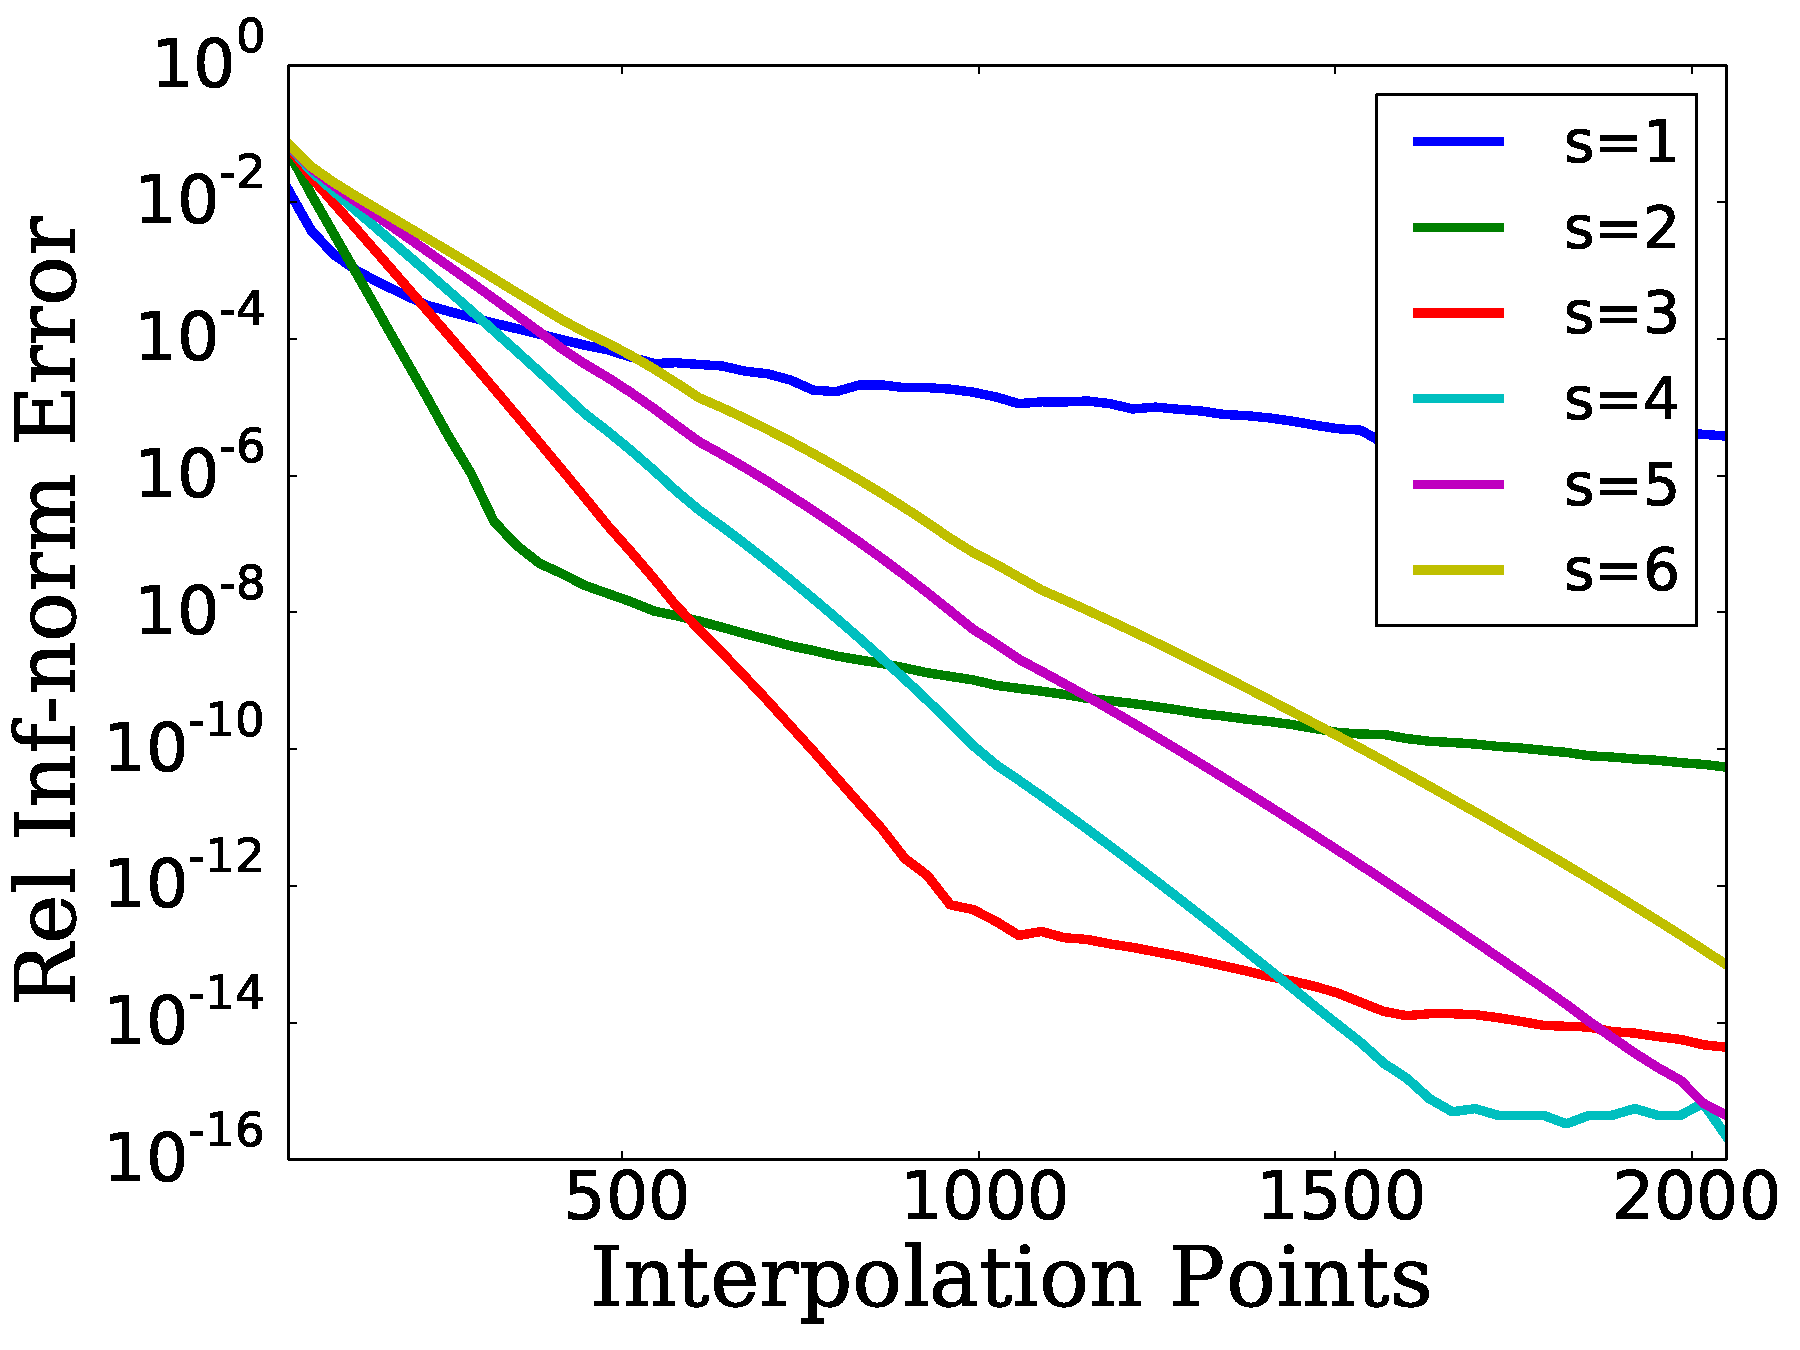
\includegraphics[width=\textwidth]{plots/msn_interp_fast_2n_rough_runge_jump.pdf}
    \caption{MSN Interpolation}
    \end{subfigure}

    \begin{subfigure}{0.45\textwidth}
    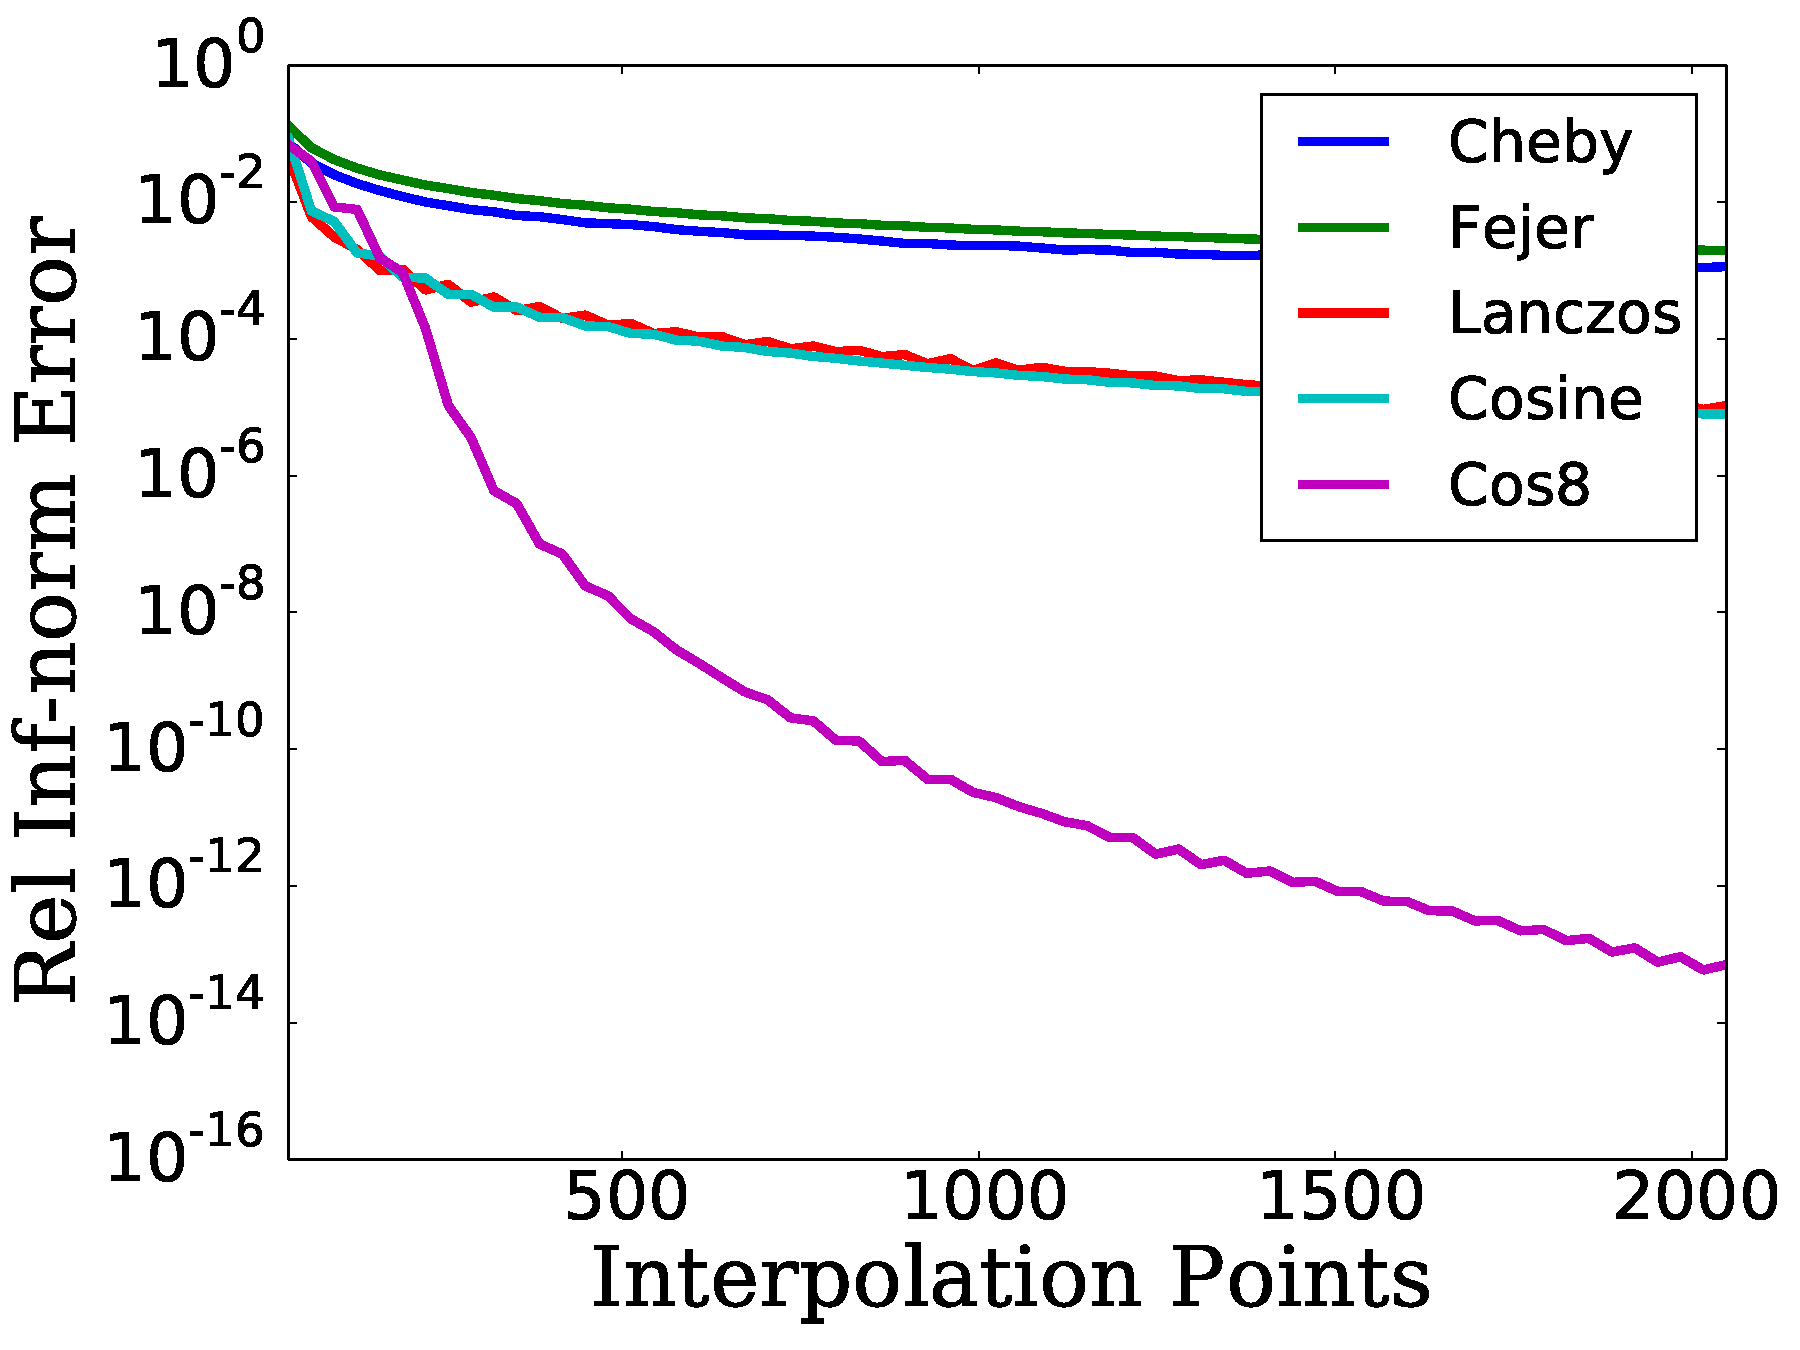
\includegraphics[width=\textwidth]{plots/cheby_interp_filter_rough_runge_jump.pdf}
    \caption{Filters, Plot 1}
    \end{subfigure}
    \begin{subfigure}{0.45\textwidth}
    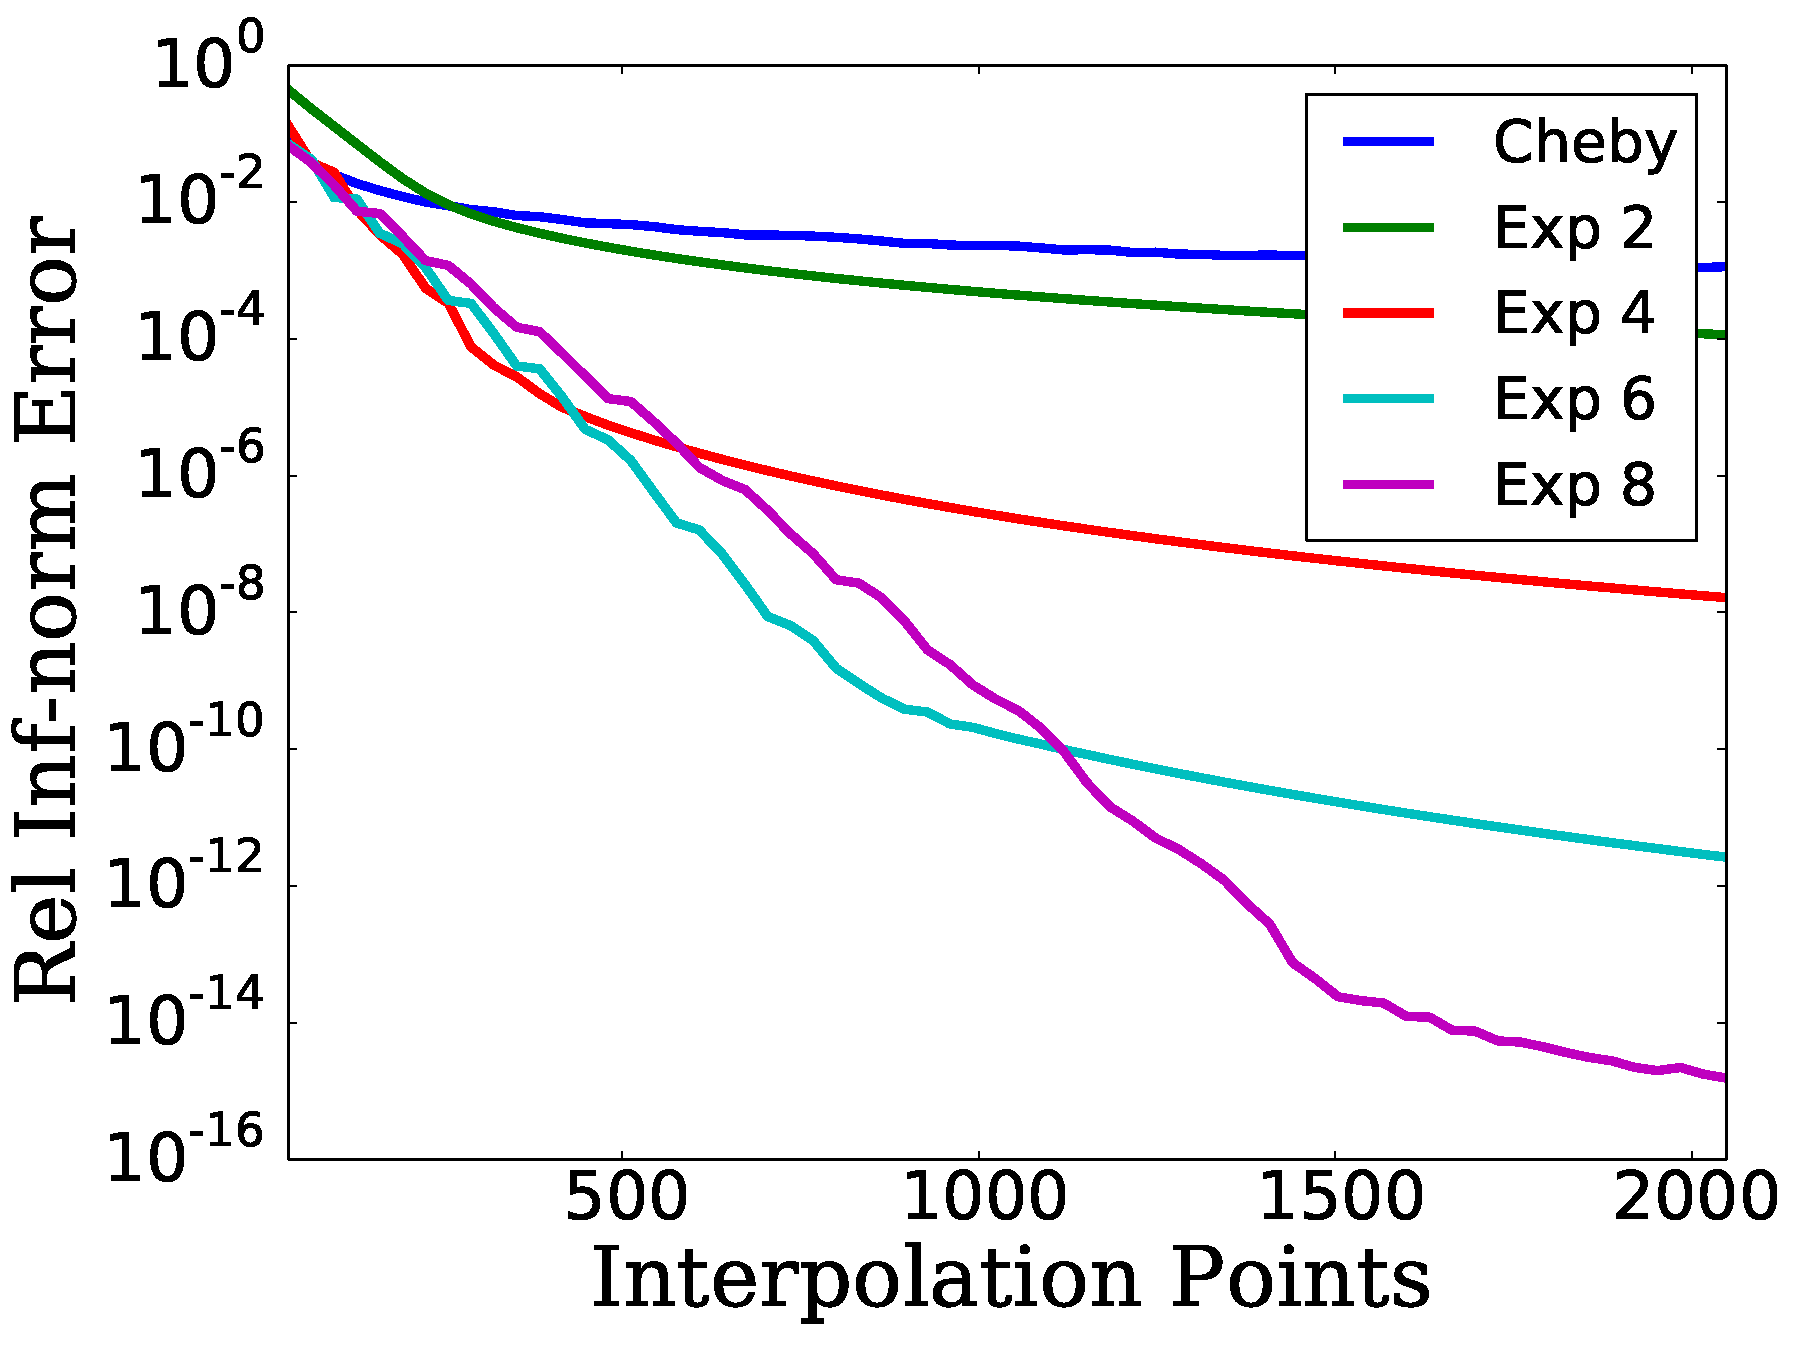
\includegraphics[width=\textwidth]{plots/cheby_interp_filter_2_rough_runge_jump.pdf}
    \caption{Filters, Plot 2}
    \end{subfigure}
\caption[Rough Interpolation Comparison: Runge Jump Function]{
MSN interpolation and Chebyshev filtering results of the Runge jump
function $R$ for various $s$ values and filters.
We include standard Chebyshev interpolant in both filter examples for reference.
}
\label{fig:rough_comparison_runge_jump}
\end{figure}



